\begin{spacing}{1.3}

    \section{Introduction}

    Let's first define(informally) what is a {\bf Greedy Algorithm}. Consider for a problem 
    that requires us to find some kinds of {\it optimal solutions}, and to find it, 
    we always makes the choice that {\it looks best at current moment}, and choose it as 
    a part of our final solution.

    This idea may sound natural, simple, and even runs efficiently. Indeed it is, however, 
    one may alert that this strategy doesn't always give us the optimal solution 
    {\it of the whole problem}(we only make optimal choice at each step, we cannot guarantee 
    the solution is still optimal after all steps). We will see some problems that greedy 
    algorithm fails to find optimal.

    As you can see, greedy algorithm is really easy, while the hardest part is how to formally
    {\it prove} it. You must convince other people that your greedy algorithm is able to 
    find {\it global optimal solution} by simply grab {\it optimal solution at each step}.
    We will cover three different kinds of problems(except for Huffman Coding, this is a special one) 
    where greedy algorithm performs well, and the first two have similar proof of correctness,
    while the third one has a totally different proof.
    (You may be required to redo the proof or adapt the proof to another similar 
    problem in homework/exam)


    \section{Interval Scheduling}

    {\bf Problem:} Given $n$ jobs, where job $j$ starts at time $s_j$ and finishes at $f_j$.
    We say two jobs $i$ and $j$ are {\it compatible} or {\it not overlap} if their time intervals 
    $(s_i, f_i)\cap (s_j, f_j) = \emptyset$. Our goal is to find the maximum-size subset
    of {\it mutually compatible} jobs.
    \begin{center}
        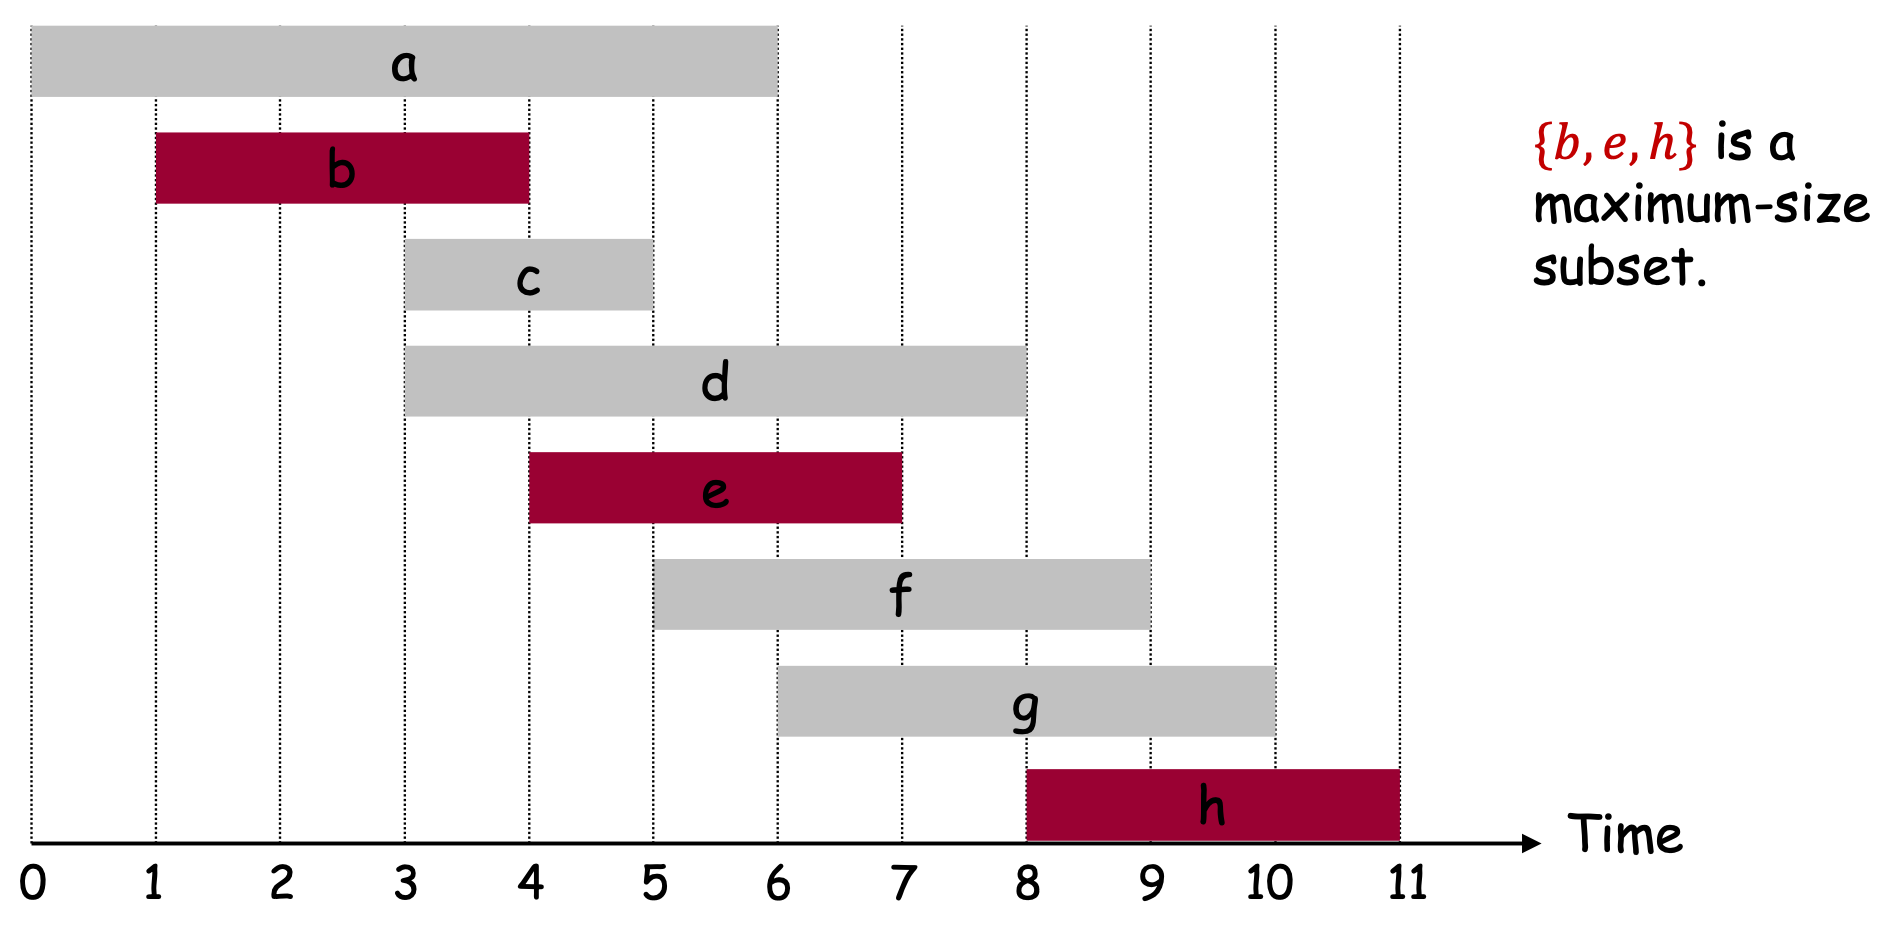
\includegraphics[scale=0.35]{images/07-interval-example.png}
    \end{center}
    In the example above, $\{b,e,h\}$ is a maximum-size subset, since you cannot find 
    a subset of size more than 4 and the jobs in that subset are mutually compatible.

    We consider to solve this problem by greedy, that is, given some jobs, we need 
    to make the best choice at current timestamp, that could make the size of subset maximized.
    So how can we maximized it? Consider choosing a job if it is compatible with all previous ones 
    that we've already taken, and not choosing it otherwise. In this way we achieve what we said that 
    ``make the best current choice''.

    However, you may easily find a counterexample, like if we first encounter a job that overlap 
    with all other jobs, then we can choose at most one job using the strategy above. So to ensure 
    its correctness, we need to first {\it consider jobs in some order}, and then use the above method.

    This order can be hard to decide, and one may think of sort jobs by:
    \begin{enumerate}
        \item increasing order of {\it start time} $s_j$,
        \item increasing order of {\it interval length} $f_j-s_j$,
        \item increasing order of {\it fewest conflicts} of each job,
        \item increasing order of {\it finish time} $f_j$.
    \end{enumerate}

    Unfortunately, we can find(not difficult) counterexamples for first three orders:
    \begin{center}
        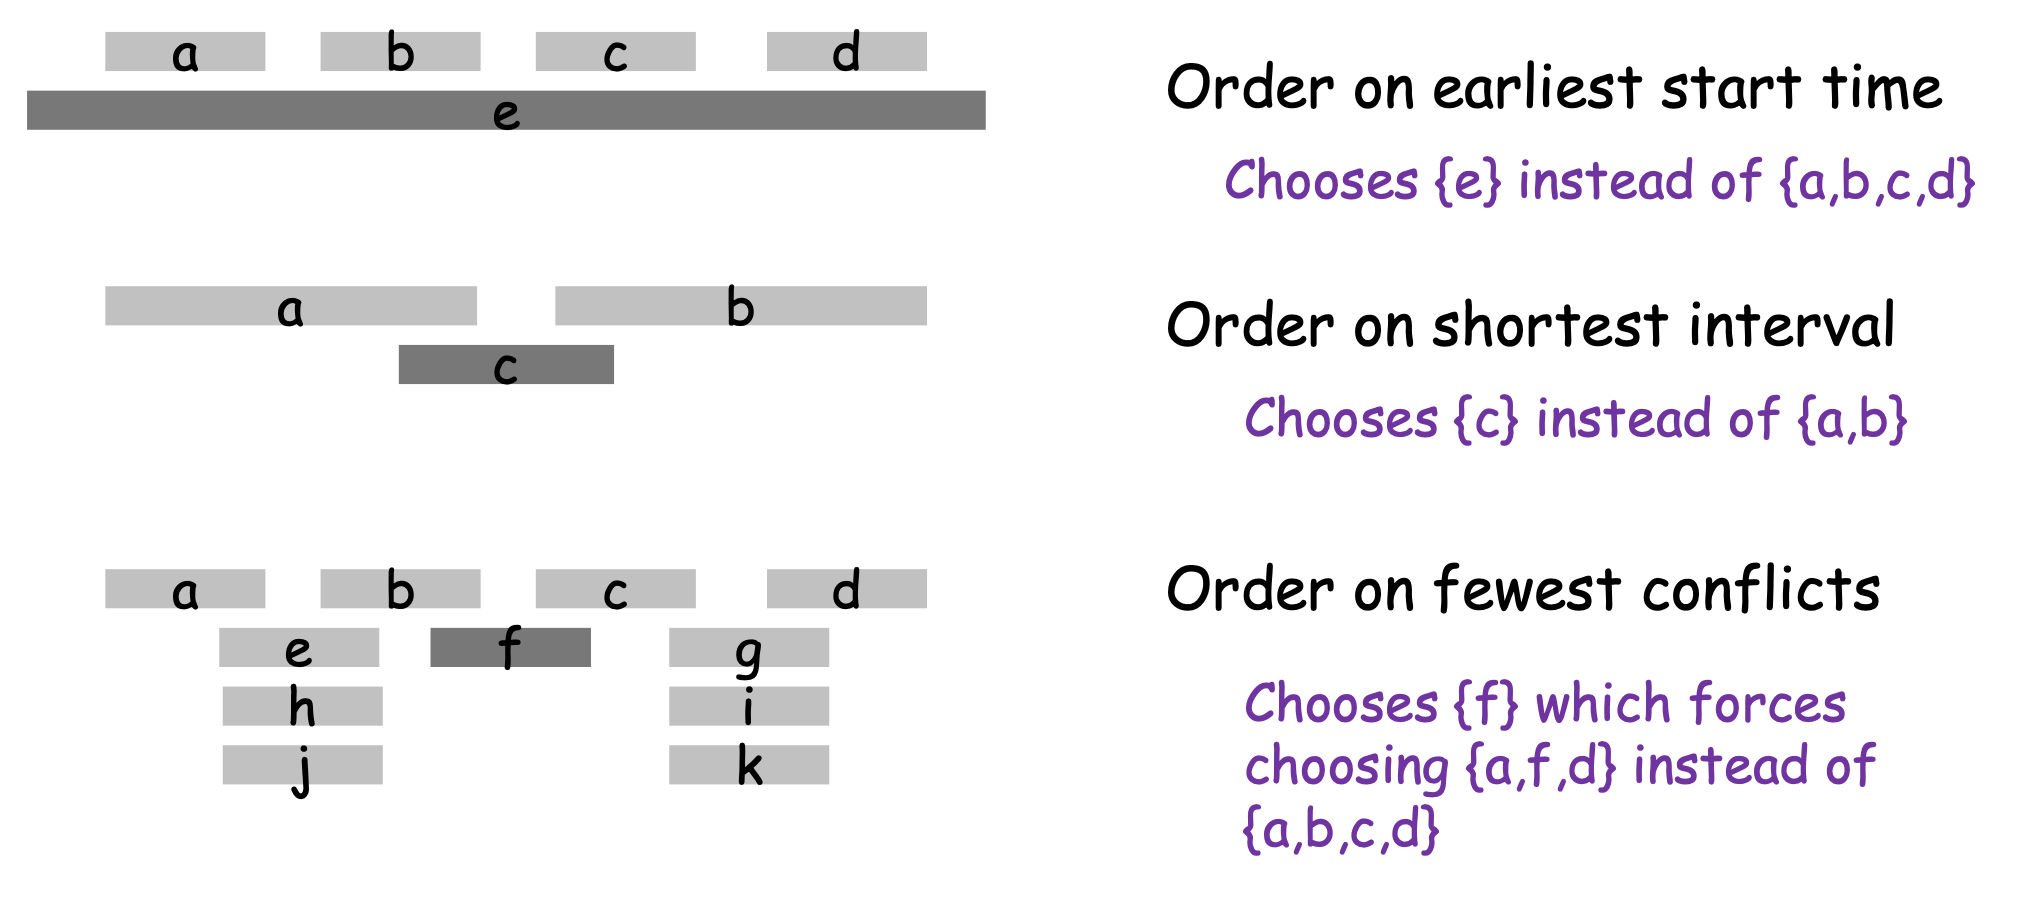
\includegraphics[scale=0.35]{images/07-interval-countereg.png}
    \end{center}

    The fourth order, i.e., sort jobs by {\it finish time}, can actually guarantee the greedy 
    algorithm to be optimal. This is not easy to find out, but the intuition is that 
    we can leave {\it maximum time} for scheduling {\it the rest of jobs}.

    You may want to review this image:
    \begin{center}
        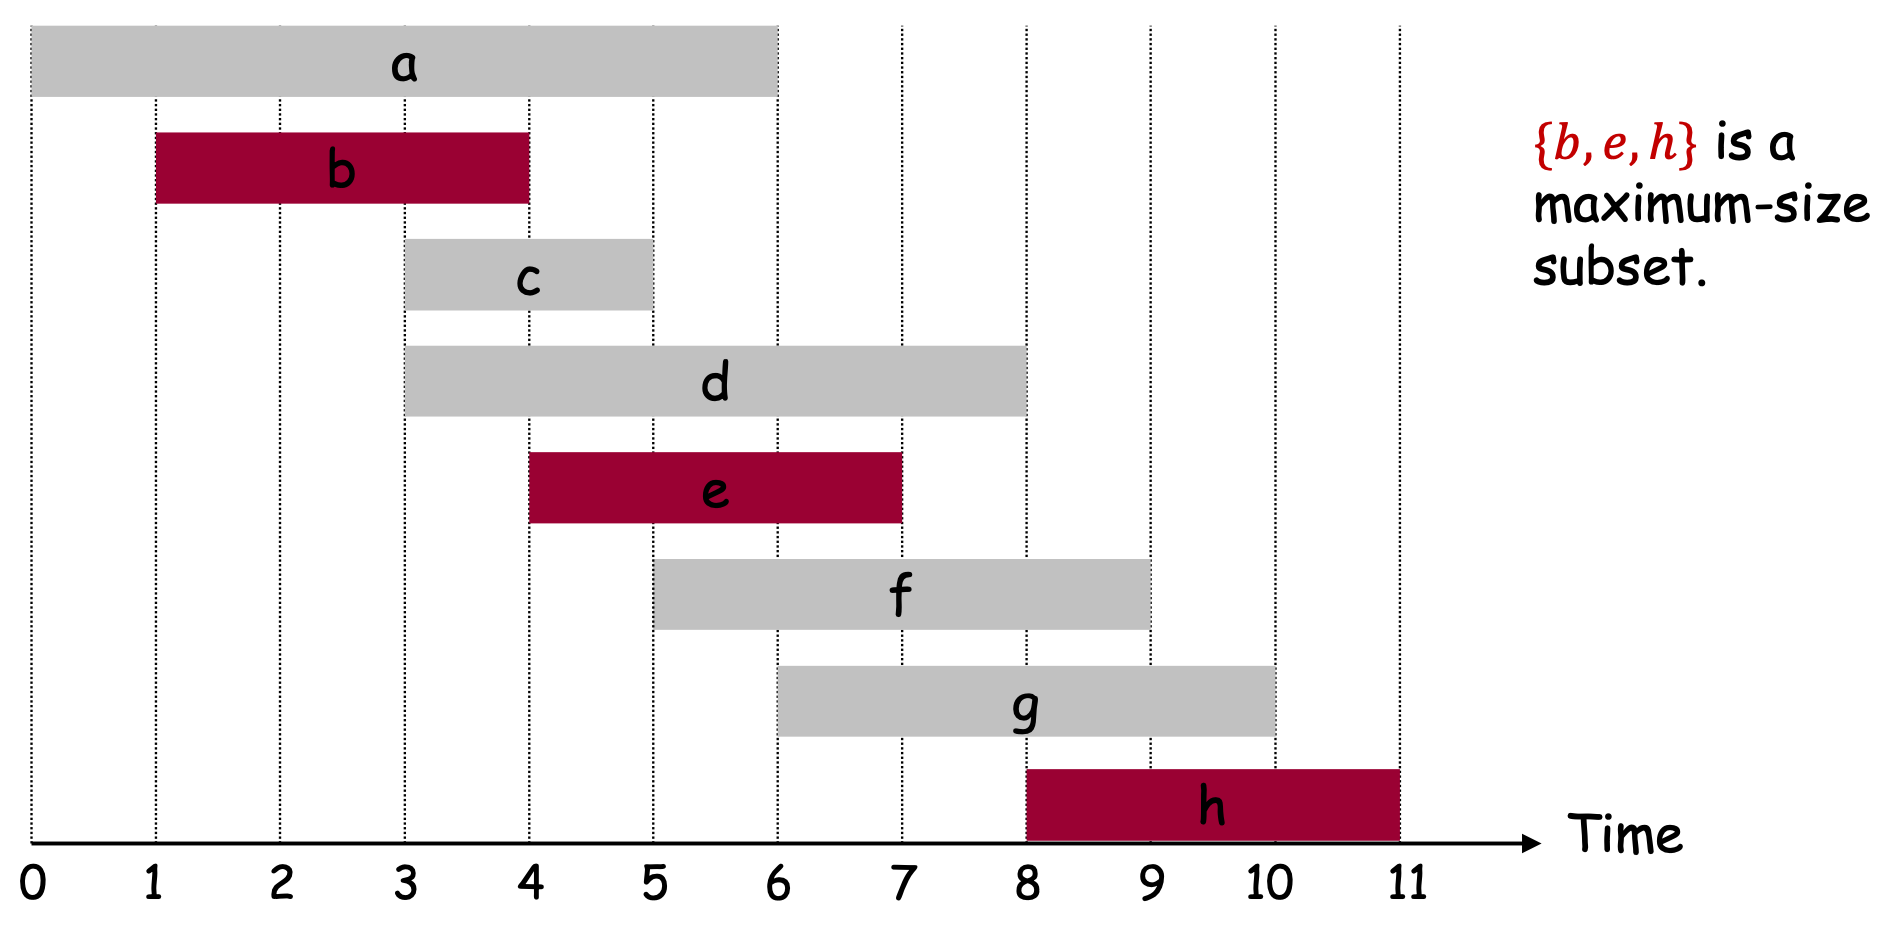
\includegraphics[scale=0.35]{images/07-interval-example.png}
    \end{center}
    We first give the code that implements this algorithm, and then formally prove it.
    
    \begin{algorithm*}
        \caption{Interval-Schedule($(s_1,f_1), \cdots, (s_n, f_n)$)}
        Sort jobs by finish time so that $f_1\le f_2\le \cdots \le f_n$

        $A\lar \emptyset$ \qquad \tcp{$A$ is the set to store the subset we found}

        $last \lar 0$   \qquad \tcp{$last$ records the {\it finish time} of last job we've chosen}

        \For{$j\lar 1$ to $n$}{
            \tcp{If job $j$ is compatiable with previous jobs, i.e., starts no earliear than 
            the finish time of last job we've chosen}
            \If{$s_j\ge last$}{
                $A\lar A\cup \{j\}$\qquad \tcp{Add job $j$ into our set}

                $last \lar f_j$ \qquad \tcp{Update $last$}
            }
        }
        return $A$
    \end{algorithm*}

    The running time of this algorithm is dominated by sorting process, which causes $\Theta(n\log n)$.

    Now let's prove the correctness of this algorithm, i.e., {\it the greedy algorithm is optimal}.

    Assume the set of jobs we get from greedy algorithm is different from an optimal set.
    Let $i_1,i_2,\cdots, i_k$ be the set of jobs found by greedy algorithm, while 
    $j_1,j_2,\cdots,j_m$ be the set of jobs in optimal solution. Our basic idea is to 
    {\it modify} optimal solution into the same as our greedy solution, while at the same time 
    {\it ensure the solution is still optimal after modification.}

    We start by finding largest possible value of $r$ such that $i_1=j_1, i_2=j_2, \cdots, i_r=j_r$,
    that is, find the last job that are the same in both sets. Thus, $i_{r+1}\ne j_{r+1}$.

    Notice in our greedy algorithm, we sort jobs by increasing of finish time, so if $i_{r+1}\ne j_{r+1}$,
    there must be job $i_{r+1}$ finishes no later than $j_{r+1}$, i.e., $f_{i_{r+1}}\le f_{j_{r+1}}$.
    \begin{center}
        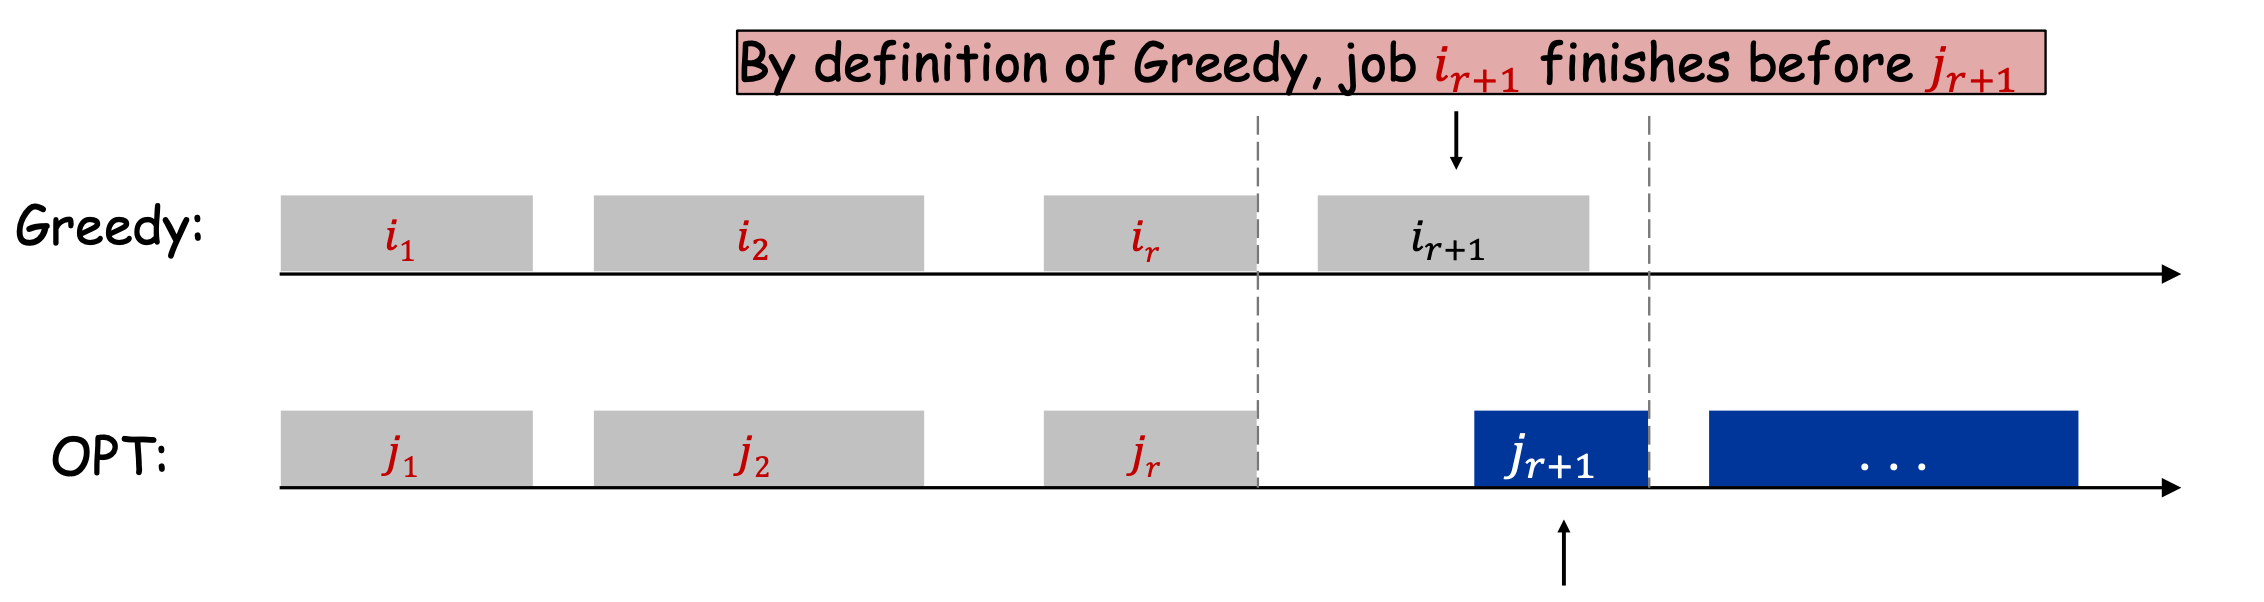
\includegraphics[scale=0.35]{images/07-interval-proof.png}
    \end{center}
    Then, we try to modify optimal solution, say, create $OPT^\star$ from $OPT$ by just replacing 
    $j_{r+1}$ with $i_{r+1}$. Notice now $OPT^\star$ is still a legal solution, the jobs are
    still mutually compatible, and $OPT^\star$ has the same size as $OPT$, so $OPT^\star$ is 
    also an optimal solution!

    Let's do this process again, until the optimal solution is the same as greedy.
    A minor problem is that they may not have the same size, i.e., $k\ne m$. 
    If this happens, the only possible is $k<m$, since $m$ is the size of optimal solution, 
    it must be the largest! However, $k<m$ is also impossible, since after replacing 
    all jobs using above method, $i_1=j_1, i_2=j_2,\cdots, i_k=j_k$. If there is 
    still jobs in optimal solution, say $j_{k+1}$, that is compatible with all previous 
    jobs, then our greedy algorithm must would have chosen that(this holds immediately 
    from our algorithm). So there must be $k=m$.


    \vspace{0.5in}
    \section{Knapsack}

    {\bf Problem:} Given $n$ items, where item $i$ has weight $w_i$ and value $v_i$.
    You now only has a knapsack that can holds weight at most $W$, you want to fill 
    your knapsack with as much {\it value} as possible. Notice in this problem an item 
    can be {\it partially used}, like each item is some liquid.

    The idea is quite simple: since we can partially use an item, we just first choose 
    items with largest ``value-weight ratio'', i.e., largest $\dfrac{v_i}{w_i}$.
    If the bag is full, we stop choosing, otherwise, we repeat the process 
    on remaining items.

    \newpage
    \begin{algorithm*}
        \caption{Fractional-Knapsack($w_1, v_1, w_2, v_2, \cdots, w_n, v_n, W$)}
        Sort items so that $\dfrac{v_1}{w_1}\ge \dfrac{v_2}{w_2}\ge \cdots \ge \dfrac{v_n}{w_n}$

        $w\lar W$\qquad \tcp{$w$ records how many {\it more} weight can the knapsack hold}

        \For{$i\lar 1$ to $n$}{
            \tcp{If $w_i\le w$, we can choose whole item, otherwise, we can only choose partial}
            \eIf{$w_i\le w$}{
                $x_i\lar 1$\qquad \tcp{$x_i$ records how much of the item is chosen, 1 means whole}

                $w\lar w-w_i$\qquad \tcp{update remaining capacity of the knapsack}
            }{
                $x_i\lar w/w_i$\qquad \tcp{choose partial}

                return \qquad \tcp{No need to update $w$, since we are already done}
            }
        }
        return
    \end{algorithm*}

    Again, its running time depends on the sorting process, which is $\Theta(n\log n)$.

    To prove the correctness of this greedy algorithm, we can assume $\disp \sum_{i=1}^n w_i\ge W$, 
    i.e., the knapsack is fully packed. Otherwise, the algorithm just takes all items thus 
    is trivially optimal.

    Again we will use the technique in last example, let the greedy solution be 
    $G=(x_1,x_2,\cdots, x_k, 0, \cdots, 0)$, where for $i<k, x_i=1$, since we fully take those items,
    and for $k$-th item, $0\le x_k\le 1$, since we may or may not fully take it, and 
    for $i>k, x_i=0$, since they are not so ``valuable'' and we didn't take it.
    Also consider some optimal solution $OPT=(y_1,y_2,\cdots, y_n)$. Note that since 
    both of them must fully pack the knapsack, there must be:
    $$\sum_{i=1}^k x_i w_i=\sum_{i=1}^n y_i w_i = W$$

    Again, we find the first item $i$ where $G$ and $OPT$ differ:
    
    \begin{tabular}{ccccccccccccc}
        $G$ & $=$ & $x_1$ & $x_2$ & $x_3$ & $\cdots$ & $x_{i-1}$ & {\blue $x_i$} & $\cdots$ & $x_k$ & $\cdots$ & 0 & 0\\
        $OPT$ & $=$ & $x_1$ & $x_2$ & $x_3$ & $\cdots$ & $x_{i-1}$ & {\blue $y_i$} & $\cdots$ & $y_k$ & $\cdots$ & $y_{n-1}$ & $y_n$\\
    \end{tabular}
   




    One thing worths mentioning is that if this problem is modified into ``items 
    cannot be partially used'', i.e., you can only either choose the item, or 
    not choose the item(also known as ``0/1 Knapsack Problem''), then there is no 
    greedy algorithm that yields optimal solution. We will come back to this in 
    Dynamic Programming.


    \section{Interval Partitioning}


    \section{Huffman Coding}


\end{spacing}